\section{Laboratory work implementation}

\subsection{Tasks and Points}

În cadrul lucrării au fost realizate următoarele funcționalități ale calculatorului:
\begin{itemize}
\item[•] operațiil +, -, /, *;
\item[•] operațiile  putere, radical, InversareSemn(+/-);
\item[•] operații cu numere zecimale;
\item[•] divizare proiectului în doua module - Interfața grafică(Modul GUI) și Modulul de bază(Core Module).

\end{itemize}

\end{enumerate}

\subsection{Analiza lucrarii de laborator}

	În cadrul acestei lucrări de laborator, a fost înaintată ca cerință de bază crearea unui calculator folosind interfață grafică. Limbajul ales pentru realizarea acestui proiect este C#, deoarece oferă posibilități mari de creare a interfețelor și este ușor de înușit. IDE-ul utilizat este Visual Studio.
	Inițial am creat interfața calculatorului, utilizând elementele grafice prestabilite de limbaj cu amplasarea butoanelor și chenarelor necesare. Ulterior, am modificat setările implicite ale elementelor, personalizându-le. 
	Interfața conține:
	\begin{itemize}
	\item 21 de butoane active;
	\item un textbox unde apare informația tastată pe butoane.
	\end{itemize}
	
	\textbf{Butonul "+"}
	
	this.plusButton.FlatStyle = System.Windows.Forms.FlatStyle.Flat;
	
    this.plusButton.Location = new System.Drawing.Point(185, 42);
    
    this.plusButton.Name = "plusButton";
    
    this.plusButton.Size = new System.Drawing.Size(42, 34);
    
    this.plusButton.TabIndex = 0;
    
    this.plusButton.Text = "+";
    
    this.plusButton.UseVisualStyleBackColor = true;
    
    this.plusButton.Click += new System.EventHandler(this.plusButton_Click);

	
	\textbf{Butonul "="}
	
	this.equalButton.FlatStyle = System.Windows.Forms.FlatStyle.Flat;
    
    this.equalButton.Location = new System.Drawing.Point(185, 176);
    
    this.equalButton.Name = "equalButton";
    
    this.equalButton.Size = new System.Drawing.Size(42, 30);
    
    this.equalButton.TabIndex = 1;
    
    this.equalButton.Text = "=";
   
   this.equalButton.UseVisualStyleBackColor = true;
   
   this.equalButton.Click += new System.EventHandler(this.equalButton_Click);
   
  
   \textbf{Butonul "x^2"}
   
   
   this.putButton.FlatStyle = System.Windows.Forms.FlatStyle.Flat;
   
   this.putButton.Font = new System.Drawing.Font("Microsoft Sans Serif", 10F, 
   
   System.Drawing.FontStyle.Regular, System.Drawing.GraphicsUnit.Point, ((byte)(204)));
   
   this.putButton.Location = new System.Drawing.Point(185, 10);
   
   this.putButton.Name = "putButton";
  
   this.putButton.Size = new System.Drawing.Size(41, 32);
   
   this.putButton.TabIndex = 5;
   
   this.putButton.Text = "x^2";
   
   this.putButton.UseVisualStyleBackColor = true;
   
   this.putButton.Click += new System.EventHandler(this.putButton_Click);
   
   \textbf{Butonul "x^(1/2)"}
   
	this.radButton.FlatStyle = System.Windows.Forms.FlatStyle.Flat;
    
    this.radButton.Font = new System.Drawing.Font("Microsoft Sans Serif", 13F, 	
    
    System.Drawing.FontStyle.Regular, System.Drawing.GraphicsUnit.Point, ((byte)(204)));
    
    this.radButton.Location = new System.Drawing.Point(122, 10);
    
    this.radButton.Name = "radButton";
    
    this.radButton.Size = new System.Drawing.Size(55, 63);
    
    this.radButton.TabIndex = 4;
    
    this.radButton.Text = "^1/2";
    
    this.radButton.UseVisualStyleBackColor = true;
    
    this.radButton.Click += new System.EventHandler(this.radButton_Click);
    
\subsection{Imagini}

\begin{figure}[!ht]
\centering
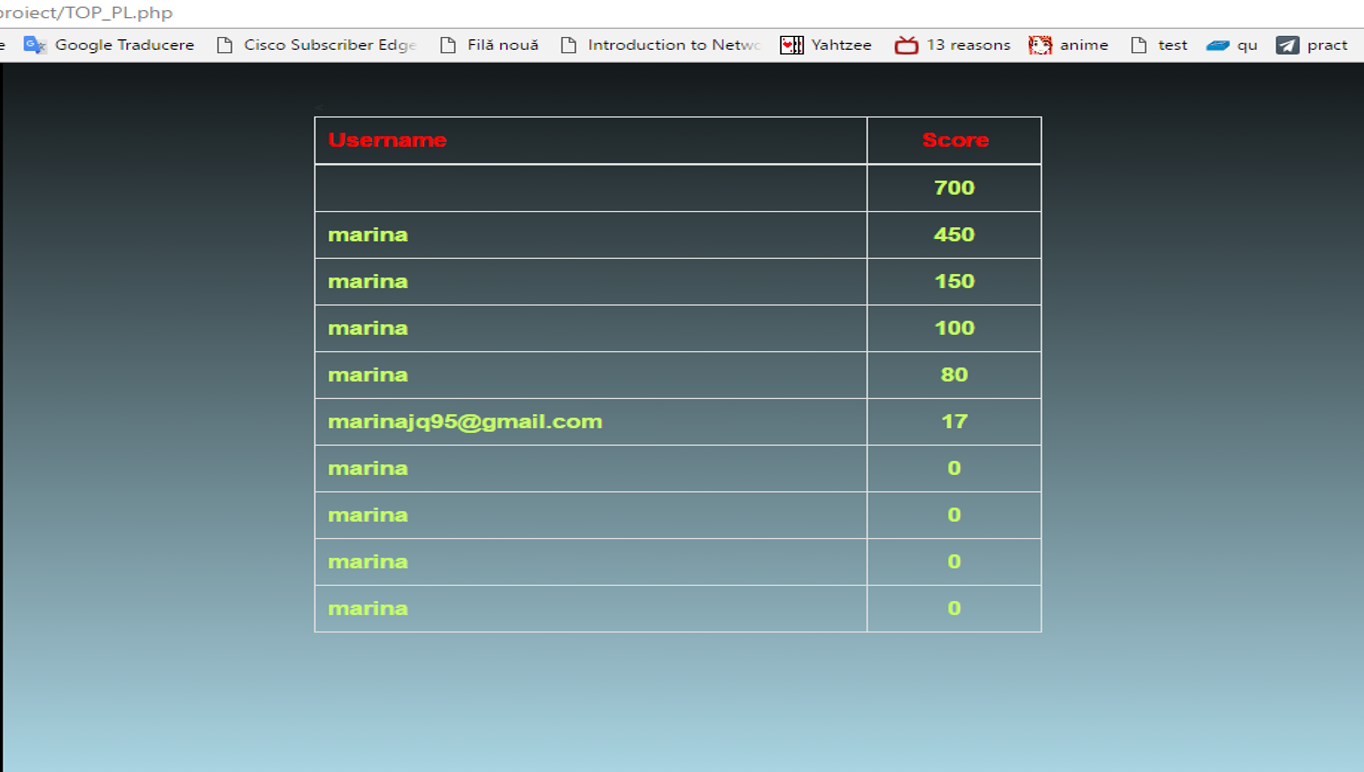
\includegraphics[width=0.3\textwidth]{1}
\caption{Interfața calculatorului, \cite{ImRef}}
\label{Im_label}
\end{figure}

\begin{figure}[!ht]
\centering

\includegraphics[width=0.3\textwidth]{2}
\caption{Radical din 52, \cite{ImRef}}
\label{Im_label}
\end{figure}

\begin{figure}[!ht]
\centering
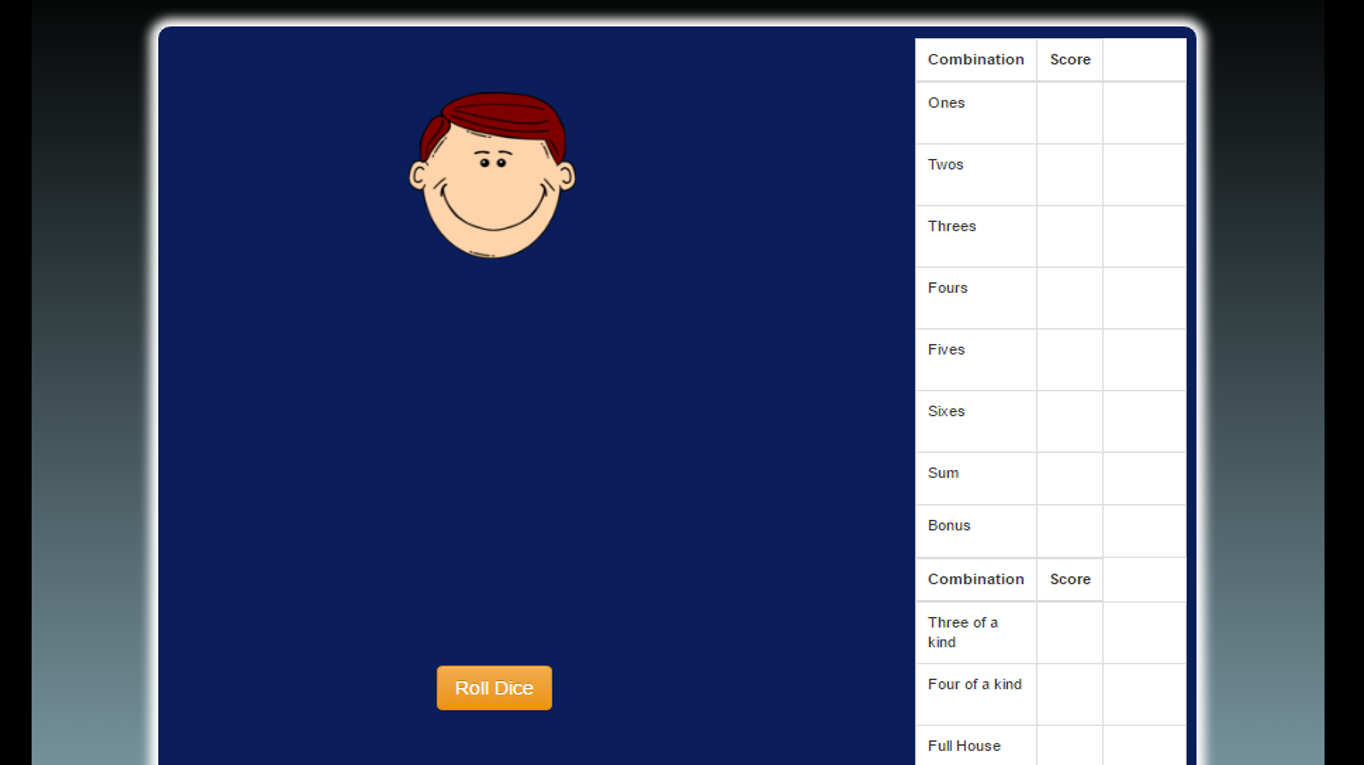
\includegraphics[width=0.3\textwidth]{3}
\caption{Patratul lui 14,23 \cite{ImRef}}
\label{Im_label}
\end{figure}


\begin{figure}[!ht]
\centering

\includegraphics[width=0.3\textwidth]{4}
\caption{Utilitatea butonului C \cite{ImRef}}
\label{Im_label}
\end{figure}

\clearpage